\documentclass{report}
\usepackage[utf8]{inputenc}
\usepackage[T1]{fontenc}
\usepackage{indentfirst}
\usepackage{fancyhdr}
\usepackage[french]{babel}
\setlength{\textwidth}{155mm}
\setlength{\textheight}{255mm}
\usepackage{wrapfig}
%\setlength{\evensidemargin}{0mm}
%\setlength{\oddsidemargin}{5mm}
\setlength{\headheight}{0mm}
\setlength{\headsep}{0mm}
\setlength{\topmargin}{-10mm}
\renewcommand{\contentsname}{\hspace*{-8mm} Table des Matières}
\usepackage{geometry}
\usepackage{graphicx}
\usepackage{url}
\geometry{
left=22mm,
right=22mm,
top=15mm,
bottom=15mm,
foot=10mm
}
\renewcommand{\thesection}{\Roman{section}}

\begin{document}
\noindent
Bon William \hfill 23 Juin 2013\\
Ernewein Audrey\\
Finck Damien\\
Goddet Marie-Hélène\\
Vanhoutreve Renaud

%\vspace{10mm}
\vfill
\begin{center}
{\Large Université de Strasbourg --- Licence informatique}

\bigskip
{\Large Projet 140H}
{\Large Androworms}
\bigskip


\includegraphics[scale=0.8]{images/splash}

\end{center}
\vfill
\newpage
%\vspace{10mm}
\tableofcontents
\newpage

\newpage

\section{Introduction}
\bigskip

Dans le cadre du projet 140h à sujet libre, nous avons choisi de faire
une application pour Android, un jeu de plate-forme.
Les projets de jeux vidéo sont souvent mal estimés. Bon nombre de
personnes pensent que c’est un jeu d’enfant de créer un jeu et pourtant
cela est rarement le cas. Certains développements de jeux vidéo peuvent
présenter des aspects plus complexes que des programmes basiques.
En effet, il faut constamment faire attention à ne pas utiliser toutes
les ressources disponibles : la partie graphique et les performances
techniques étant généralement plus gourmands que pour des programmes
normaux. De plus, les ralentissements dans le jeu imputent fortement la
jouabilité, ce qui dérangera l’utilisateur final. La gestion des
ressources représente donc un des objectifs principaux du projet.

\bigskip

Pour ce projet, nous avons décidé de mettre l’accent sur les quatre
objectifs ci-dessous :
\begin{itemize}
\item l’ergonomie : une interface graphique facile à utiliser
\item la jouabilité : un jeu simple et fonctionnel
\item les performances : un temps de réponse très faible et pas de latence 
\item le caractère innovant du projet
\end{itemize}


\newpage

\section{Choix du sujet}
\bigskip

\subsection{Les spécifications que nous avons choisies}
\bigskip


Le choix d’un projet mobile s’est imposé pour plusieurs raisons. 
En effet, ce projet nous est apparu comme une occasion de découvrir
le développement sur smartphone, aucun membre du groupe n’ayant eu
l’occasion d'effectuer de développement mobile jusque-là. De plus,
ces cinq dernières années, l'essor des smartphones a quelque peu
bouleversé le marché des logiciels informatiques en plaçant le mobile
en première place et rendant le développement mobile un métier d’avenir.

L’acquisition de nouvelles compétences nous a décidés à relever ce
challenge : découvrir la programmation mobile à travers ce projet. 
Aucun membre de l’équipe n’ayant de smartphone sous Windows Phone ou
iOs, le choix du système d’exploitation s’est rapidement tourné vers
Android. Pour des raisons budgétaire, il n’était pas envisageable
d’acquérir de nouveaux matériels.
Au final seul Renaud, ne disposant pas de smartphone ou tablette, a
dû utiliser intégralement la machine virtuelle Android pour réaliser
ses développements et tests.

Les spécifications issues du cahier des charges et utilisées dans
notre application sont les suivantes :
\begin{itemize}
\item un développement Java
\item un développement uniquement sous Android 
\item un jeu de plateforme s’appuyant sur le célèbre jeu « Worms »
\item la possibilité de jouer en multi-joueurs
\item l’utilisation des capteurs des smartphones
\end{itemize}

\subsection{Les contraintes du sujet}
\bigskip


Lors de la définition de notre projet, nous avons compris que l’objectif
de ce projet était de faire un site internet ou une application mobile
selon le travail effectué en entreprise. Nous sommes plusieurs dans le
groupe à participer à la création de sites web dans le cadre de notre
travail, c’est pourquoi nous avons choisi Android, que nous n’avons
jamais utilisé, afin de respecter l’objectif du projet.

Nous avons également compris que vous attentiez de nous un projet sur
un sujet inconnu avec de réelles contraintes techniques. A travers ce
projet, nous avons dû mettre en avant nos capacités d’adaptation et de
prises de décisions pour réussir à atteindre nos buts malgré les
difficultés. En effet, l’intégration des API sociales pour pouvoir
partager le score des joueurs a été un réel challenge que nous
développerons dans la suite du rapport.

Dans cette optique de travail, nous nous sommes intéressés aux
capacités techniques de nos appareils, en utilisant les capteurs du
téléphone comme la caméra, le « touch » et « multi-touch » sur l’écran,
le son, le vibreur et l’accéléromètre.

Lors de la démonstration de mi-projet, vous nous avez suggéré
l’utilisation de SDK pour nous aider dans la conception de ce projet. 
Malgré cette demande, cela n’a pas pu être réalisé pour plusieurs
raisons :
\begin{itemize}
\item L’utilisation des composants graphiques internes à Android
représentaient déjà un véritable challenge pour nous.
\item Il existe peu de SDK pour les applications Android 2.3.x et plus.
\item Il faut beaucoup de temps pour comprendre et apprendre à
utiliser un SDK. Ce temps rajouté à l’apprentissage d’Android, aurait
représenté une part trop importante de notre projet.
\item Un nouvel outil, c’est également plus de difficultés et des bugs
à prévoir, mais aussi des limitations d’usage qu’on peut rencontrer
en cours d’utilisation.
\item Le SDK n’aurait pas répondu exactement à nos demandes
\item Nous avons choisi de découvrir Android tel quel sans surcouche
dans le cadre de ce tout premier projet d’application mobile.
\end{itemize}

\newpage

\section{Analyse du sujet}
\bigskip


\subsection{Moyens techniques}
\bigskip


\subsubsection{Choix du langage et de l'API}

Pour notre premier projet Android, nous avons décidé d’utiliser le SDK
Android compatible avec Android 2.3.x ou supérieur afin d’obtenir une
compatibilité avec la majorité des appareils Android enregistrés à ce
jour, c’est à dire 84,2\%.

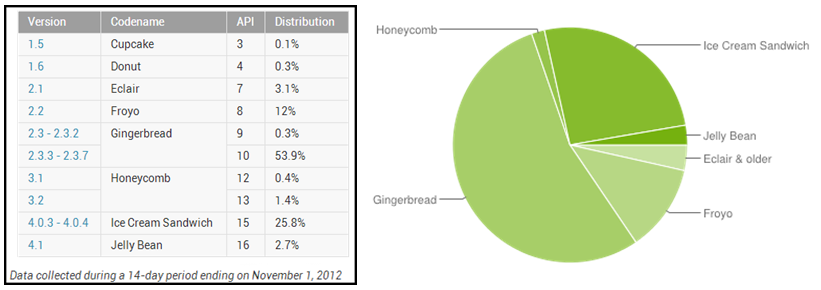
\includegraphics[scale=0.75]{images/graph1}

Cependant, entre septembre début du projet et juin, l’état du marché a
énormément bougé.
Plus de 50\% des mobiles utilisent actuellement une version 4.0.x ou
supérieur, ce qui ne justifierait plus forcément notre choix de départ.
Ceci s’explique par une technologie relativement récente entraînant la
sortie de mises à jour fréquentes et surtout la venue de nombreux mobiles
rendant les vieilles versions obsolètes.

L’anticipation de cette évolution et l’utilisation de la version 4.0.x
et de son API nous aurait grandement simplifié le développement.
Dorénavant, le développeur n’est plus obligé de tout redévelopper de
lui-même, de qui engendre un gain de temps phénoménal.
\bigskip


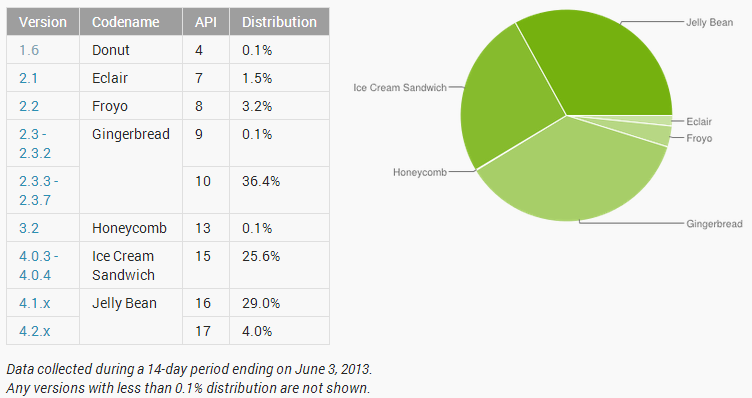
\includegraphics[scale=0.75]{images/graph2}

\subsubsection{L'environnement de développement}
Afin d’uniformiser l’environnement de développement entre tous les
membres de l’équipe, une documentation d’installation et configuration
de l’IDE et des plugins a été créée.
D’un commun accord, il a été décidé d’utiliser « Eclipse » que ce soit
sous Windows ou Linux, auquel on a rajouté le SDK Android et le plugin
du gestionnaire de version.

\subsubsection{Le gestionnaire de version}

Afin de rendre le code source disponible, nous avons décidé de
l’héberger sur Google Code à l’adresse suivante :
\url{http://code.google.com/p/androworms}.
Ce choix nous a permis d’utiliser le tracker intégré, permettant
d’affecter des tâches aux différents membres du groupe, que ce soit pour
des bugs ou des demandes d’évolutions
(\url{http://code.google.com/p/androworms/issues/list}). Cette
fonctionnalité permet l’envoi direct d’un mail à la personne en charge
de la tâche.

N’ayant jamais eu de problème de compatibilité entre Eclipse et SVN,
son choix comme gestionnaire de version s’est rapidement imposé.

\subsubsection{La gestion de la qualité du code source}

Dès le début du projet, Sonar (\url{http://www.sonarqube.org/}) a été
installé sur un serveur tiers afin de contrôler et améliorer la qualité
du code source.
Cette plate-forme de contrôle continu effectue une analyse à chaque
commit et renvoie le résultat en moins d’un minute.

Un code propre et facile à maintenir est absolument nécessaire,
essentiellement lorsqu’on est plusieurs à intervenir dessus. En effet,
il n’est pas toujours évident de comprendre le code des autres, mais
cela peut être encore plus contraignant si le code n’est pas propre ou
correctement indenté.

Notre instance de Sonar est disponible à l’adresse suivante :
\url{http://doc.petrolkiwi.net/}.

\subsubsection{Communication}

La communication au sein du groupe n’a pas toujours été facile.
Principalement en raison de l’emploi du temps de chacun, mais également
en raison de la division par groupe pendant les TD/TP. Au final très peu
de travail personnel en commun.

D’autres moyens de communications ont été utilisés :
\begin{itemize}
\item des mails, plus de 270, à chaque fois adressés à toute l’équipe
\item la création d’issue tracker individuel
\item des commentaires sur les commits sous forme de mails individuels.
\item des réunions pour les grosses décisions : rédaction du cahier des
charges, élaboration de la vidéo finale, etc...
\end{itemize}

\newpage

\section{Moyens techniques mis en place}
\bigskip


\subsection{Début du projet}
\bigskip


Pour commencer le projet, nous avons fait plusieurs réunions pour
choisir le sujet du projet et le définir précisément. Nous avons
également à cette occasion choisi les technologies employées.
Ensuite nous avons découpé le travail à faire et réparti les tâches
entre les différents membres de l’équipe.

Répartition des taches:

\begin{tabular}{|c|c|c|c|c|c|c|c|}
\hline
{\bf Tâche } & {\bf William } & {\bf Audrey } & {\bf Damien } & {\bf Marie-Hélène } & {\bf Renaud }\\
\hline
{IHM des menus} & {} & {} & {X} & {} & {}\\
\hline
{IHM du jeu} & {} & {} & {} & {} & {} \\
{(graphismes)} & {} & {X} & {} & {} & {} \\
\hline
{IHM du jeu} & {} & {} & {} & {} & {}\\
{(gestion des composants)} & {} & {X} & {X} & {X} & {} \\
\hline
{Editeur de carte} & {X} & {} & {} & {} & {} \\
\hline
Déplacement des perso &&&&&\\
(déplacement + &&&&& X\\
gestion de la collision + &&&&&\\
 gravité) &&&&&\\
\hline
{Armes (trajectoire)} & {} & {} & {} & {} & {X} \\
\hline
{Jeux tour à tour} & {X} & {} & {} & {} & {X} \\
\hline
{API (Facebook,} & {} & {} & {} & {X} & {} \\
{ Google+, Twitter)} & {} & {} & {} & {} & {} \\
\hline
{Gestion du réseau} & {} & {} & {X} & {X} & {} \\
{(Bluetooth)} & {} & {} & {} & {} & {} \\
\hline
{Intelligence Artificielle} & {} & {} & {} & {} & {X}\\
\hline
{Intégration continue} & {} & {} & {X} & {} & {}\\
{et Sonar} & {} & {} & {} & {} & {}\\
\hline
\end{tabular}
\bigskip


Au début du projet, nous avons dû mettre en place le dépôt Google et
installer Sonar sur un serveur. Ensuite, nous avons chacun étudié le
fonctionnement du SDK Android et commencé à faire des essais.

\subsection{Diagramme d’utilisation}
\bigskip


Dans un premier temps, nous avons défini notre projet et mis en place un
diagramme d’utilisation. Cela correspondait au cours « Analyse et
architecture logicielle orientée objets » que nous avons eu lors de cette
seconde année en master « Ingénierie des logiciels et des
connaissances ». Ce diagramme reflète les principales fonctionnalités
de notre application.

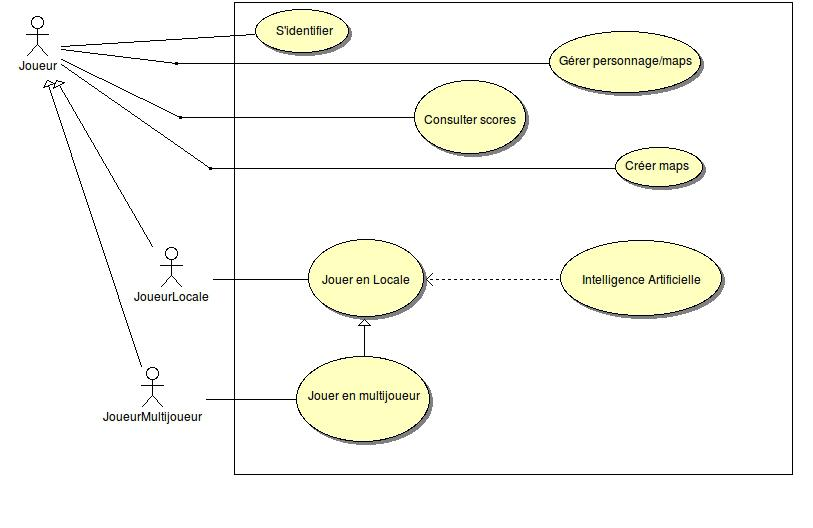
\includegraphics[scale=0.5]{images/graph3}

\subsection{Élaboration d’un diagramme de classe}
\bigskip


Lors de la spécification du projet, un diagramme de classes avait été
construit. Ce diagramme comportait un nombre de classes réduit. Étant
soucieux d’utiliser une représentation UML, le premier diagramme fût
enrichi pour obtenir la version suivante : 

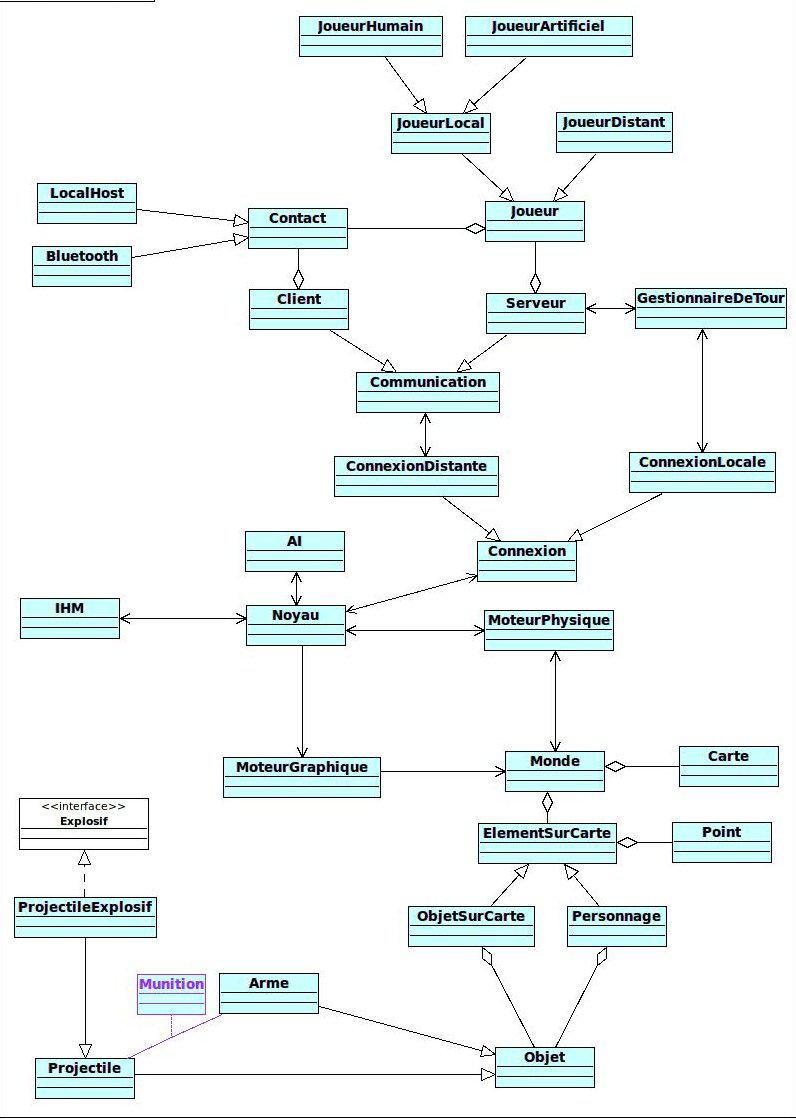
\includegraphics[scale=0.5]{images/graph4}
\bigskip

En raison de nos faibles connaissances en conception et réalisation de
jeux vidéo, nous avons eu beaucoup de mal à estimer les besoins de ce
projet. Ce schéma a donc été notre référence tout au long du projet. Sa
création a soulevé des questions importantes :

\begin{itemize}
\item Comment faire pour garder le même comportement en mode solo et
multi-joueurs ?
\item Où placer l’intelligence artificielle ? Dans la partie réseau,
afin de l’exécuter sur l’appareil le plus puissant et réduire les temps
de calcul ou l’attacher au noyau pour simplifier le développement ?
\end{itemize}

\newpage

\section{Réalisations et difficultés}
\bigskip


\subsection{Présentation du projet}
\bigskip


Le but du projet était d'acquérir des compétences complémentaires à
celle acquises en entreprise, d’où l’idée de créer un mini jeu mobile
pour Android. Ce jeu est une version modifiée du jeu bien connu « Worms »,
dans lequel deux joueurs (ou un joueur et une IA) s’affrontent en
s’envoyant des projectiles jusqu’à ce qu’un des joueurs n’ait plus de
points de vie.
Pour mener à bien ce projet, nous avons découpé le projet global en
sous projets articulés. Ci-dessous une présentation de ces sous projets
et de leur avancement.

\subsection{Architecture du projet}
\bigskip


Comme précisé dans la section précédente, le diagramme de classes a bien
guidé les développements. Cependant, il manquait de précision en raison
de notre manque de connaissances des besoins et des spécificités d’un
tel projet.

La représentation de notre programme n’a pas été modifiée durant un
long moment, pour finalement aboutir au diagramme de classes de notre
application actuelle :

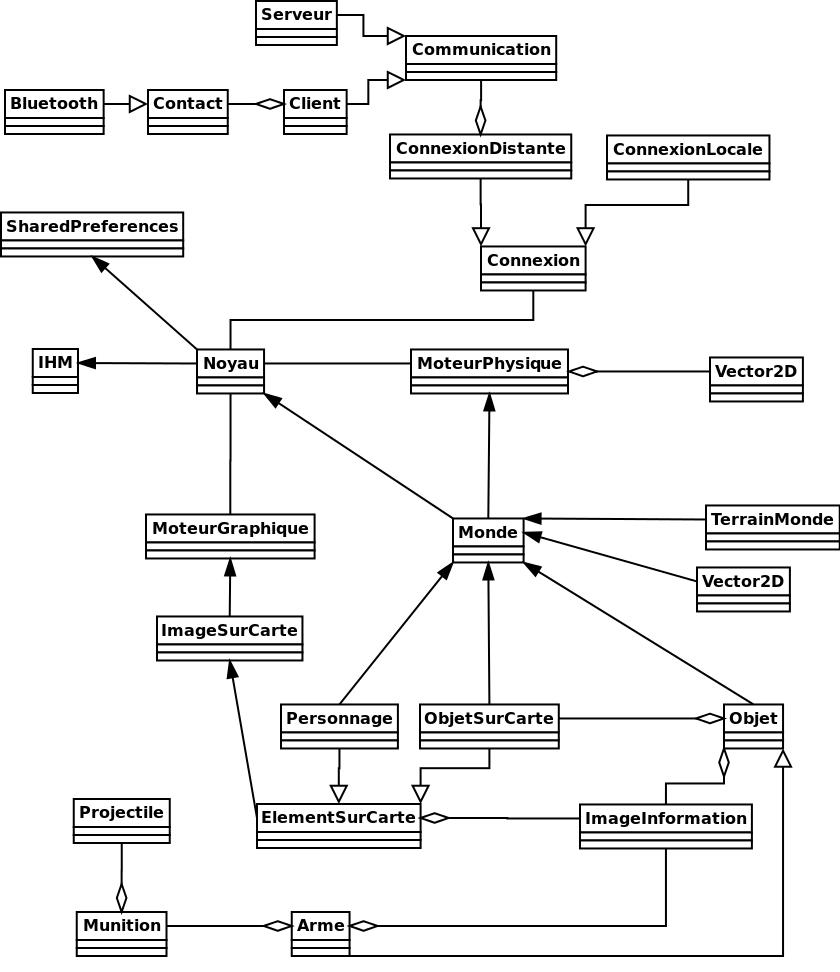
\includegraphics[scale=0.5]{images/graph5}

Dans ce schéma, les flèches noires représentent l’agrégation : les
flèches pointent vers un objet appelant l’objet d’où la flèche part.
Les losanges blancs indiquent la composition et les traits impliquent
une agrégation dans les deux sens. Seules les classes créées et utilisées
apparaissent dans le schéma afin de simplifier la lecture du schéma.

On remarque que le diagramme de classe initial à bien été respecté,
malgré quelques erreurs. Par exemple, la classe « ImageSurCarte » est
utilisé uniquement pour stocker les informations du «~Personnage~» pour
permettre son affichage. Il aurait été possible de fusionner les deux
classes afin d’en garder une seule et unique classe «~Personnage~»
accessible via le noyau.

La classe « TerrainMonde » a remplacé la classe carte, pour deux
raisons:

\begin{itemize}
\item Une autre classe « Carte » a été créée est correspond
d’avantage à la dénomination ;
\item La classe « TerrainMonde » représente plus qu’une simple
classe. En effet, on peut y trouver l’arrière-plan, le premier
plan et le terrain constitué des deux premiers items pour éviter
de recréer la carte à chaque calcul.
\end{itemize}
L’une des grosses difficultés fut de comprendre le fonctionnement
d’une interface afin d’y inclure des animations. Les animations sont
problématiques car elles nécessitent un réaffichage de l’écran sans
intervention de l’interface graphique ou de l’utilisateur. Pour les
mouvements, cela est assez simple, l’interface graphique invoque des
méthodes et les modifications sur la position du personnage s’exécutent.
Ensuite, on demande l’actualisation de l’interface et notre code
s'arrête. Là les appels sont dépilés et en raison de cette dépilation,
l’interface est réactualisée. Notre soucis était d’utiliser ce mécanisme
afin d’obtenir une animation. Ne le connaissant pas a priori, nous
étions partis sur des threads, puis sur des activités (concept expliqué
par la suite), peine perdu.

Le plus simple fut d’utiliser des classes « Runnable » mais pas de façon
traditionnelle. Les runnables sont comme des threads, or notre
problématique est de relâcher le fil d'exécution. Les Runnables ont une
gestion des messages efficaces en java et c’est ce que nous avons
utilisé. Lorsqu’il fallait faire une animation, un Runnable était créé
et appliquait un changement sur un personnage par exemple, puis lançait
un message interne en se passant en paramètre. Le fil d'exécution était
donc relâché et le mouvement du personnage était effectué.
Lorsque le message interne revenait, l’intégralité du fil d'exécution
était restaurée, permettant de redessiner l’objet sans l’intervention
de l’utilisateur ou de l’interface graphique.

Dans le diagramme ci-dessous, on voit la division de l’application en
5 « activités ». 
Une « activité » sous Android, est une section de l’application. On
utilise généralement une pile pour passer d’une application à l’autre,
mais également pour pouvoir revenir à l’application précédente (sauf
certains cas particuliers comme pour la création de la partie).

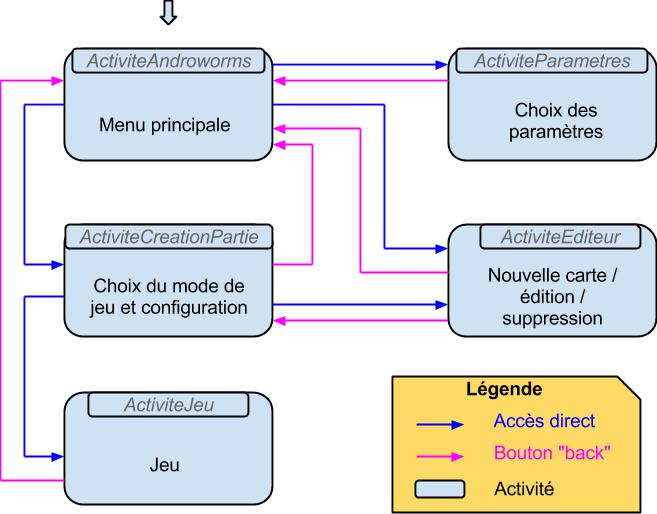
\includegraphics[scale=0.5]{images/graph6}

\subsection{L’interface utilisateur}
\bigskip


Nous avons lu les spécifications de Google sur les normes d’interface
utilisateur afin de permettre aux personnes d’avoir un retour uniforme
et une bonne expérience utilisateur sur les téléphones sous Android.
Nous avons respecté autant que possible ces contraintes en termes de
couleur, icône, ou comportement.
Le projet contient un menu qui permet d'accéder à :
\begin{itemize}
\item la création de partie en spécifiant des paramètres
\item l’éditeur de carte
\item une page qui permet de poster sur les réseaux sociaux
\item une page de paramètres
\end{itemize}

\subsection{Les graphismes}
\bigskip


En France, il n’est pas nécessaire de déposer une œuvre pour qu’elle
soit considérée comme telle et protégée. De ce fait, une majorité des
images présentes sur internet est soumise au droit d’auteur. Ce droit
protège les images de la modification, reproduction, diffusion ; elles
ne peuvent être exploitées sans l’autorisation de l’auteur.

Pour des soucis de légalité et dans l’optique d’une éventuelle
commercialisation de l’application dans le futur, nous avons décidé de
créer nos propres images.

Chaque smartphone ayant un espace mémoire différent, il a fallu créer
des images de tailles respectables et utilisables sur tous les
appareils. Une image de taille trop importante serait trop longue à
charger sur certains téléphones et pourrait créer des erreurs OOM
(mémoire insuffisante) en prenant trop de place en mémoire.

Concernant le déplacement des personnages, nous avons tout d’abord pensé
à utiliser des sprites, mais l’image aurait également été lourde en
mémoire. De plus, Android propose une propriété Animation sur les View,
permettant d'enchaîner plusieurs images à la vitesse choisie.

\subsection{Le jeu et la physique}
\bigskip


\subsubsection{Les déplacements}

Les déplacements utilisent le système de collision détaillé un peu plus
bas. Un joueur peut se déplacer, marcher, uniquement si la différence de
hauteur entre ses positions est inférieur à un certain seuil fixé. Le
personnage peut se déplacer d’un nombre fixe de pixels à gauche ou à
droite. La lenteur ressentie lors des déplacements provient des prises
de position du doigt de l’utilisateur qui sont fixes pendant un
intervalle de temps donné. Afin de fluidifier le mouvement il faudrait
diminuer cet intervalle.

\subsubsection{Les sauts et les tirs}
Les sauts et les tirs suivent la même mécanique, à la seule différence
des valeurs initiales. Pour les sauts, le vecteur initial est fixe et
défini dans l’application, alors que pour les tirs, c’est au joueur de 
définir le vecteur d’initialisation. Ensuite chaque point de la 
trajectoire est calculé, puis stocké faisant ensuite l’objet d’un 
affichage. Pour la trajectoire, un intervalle de temps fixe est choisi 
(pour l’instant 200ms) et chaque point est calculé à partir du point 
initial et du temps écoulé.

L’équation pour une position est la suivante :

$
x = P_{x} + t*V_{x} + \sum t^{2}* a_{i}
$

\bigskip

Avec :
\begin{itemize}
\item P: la position initiale
\item t: un temps donné,
\item V: un vecteur initial 
\item a: un tableau d’accélération (typiquement la gravité et le vent)
\end{itemize}

\bigskip

Pour la position suivante nous avons :

$
x = P_{x} + (t+\epsilon)*V_{x} + \sum (t+\epsilon)^{2}* a_{i}
$
\bigskip

Avec :
\begin{itemize}
\item P: la position initiale
\item t: un temps donné,
\item V: un vecteur initial 
\item a: un tableau d’accélération (typiquement la gravité et le vent)
\item $\epsilon$: le quantum de temps choisi
\end{itemize}

Les positions sur l’axe des Y se calculent exactement de la même manière. 
Pour la gravité, le vecteur initial est forcément nul, seules les 
accélérations entrant en compte. 

D’ailleurs pour ce genre d’action, il faudra faire attention à ce que le
saut, la gravité ou le tir s'arrête lorsqu’il rentre en contact avec 
les éléments du décor. En effet, l’action suit une somme de quantum de
temps, mais lorsque cette somme est grande, la nouvelle position est à
K pixels de la précédente (K >= 1). Sur la fin de la trajectoire, il 
n’y aura que peu de chance pour que le personnage effectuant un saut
atterrisse les deux pieds par terre. Il flottera sûrement dans les
airs puisque c’est la dernière position valide (position sans
collision). Il faudra ajuster la position en fonction des deux
derniers points (l’avant-dernier point valide et le dernier point
invalide). 
Pour pallier à ce problème, notre code parcourt l’ensemble des points 
formés par la droite décrite par ces deux derniers points et en déduit 
la position réelle de l’élément.

Ce fonctionnement rend la dernière position imprécise car les 
accélérations produisent généralement une trajectoire « bombée ». Cette 
imprécision reste cependant acceptable pour l’application que nous 
développons.

\subsubsection{Les collisions}
La gestion des collisions a subit un grand changement dans son 
fonctionnement depuis le début du développement.

Dans les premières versions d’Androworms, l’accent avait été mis sur les
performances limitées des appareils. C’est pourquoi la gestion des
collisions représentait un calcul très important, nous nous sommes donc
dirigés vers l’utilisation des enveloppes convexes. C’est un système
bien plus rapide que de parcourir l’ensemble des points du personnage
pour vérifier les collisions. En effet, notre bonhomme faisant 81x107
pixels (8667 pixels en tout), cette vérification devait être faite sur
chaque position lors du déplacement du personnage. 

Le souci de l’enveloppe convexe se pose lors des sauts, ces déplacements
ne se limitant pas à un pixel de côté ; des points de textures pouvaient
entrer en collision sans être détectés. 
Le système d’enveloppe convexe a finalement été mis de côté pour un
calcul exhaustif de la collision afin de pallier à toutes les
possibilités.

\subsubsection{Retour sur objectifs}

Pour la partie physique, les objectifs ont été atteints. Il est possible
de tirer, sauter et se déplacer en accord avec la physique des jeux
vidéo actuels. 

Cependant il existe un léger souci sur le mouvement de la grenade lors
d’un tir. En effet, lorsque la grenade redescend lors d’un tir direction
nord-est, il y a une accélération du mouvement. Ceci n’est pas forcément
un bug, le système de cache y ayant probablement sa part de
responsabilité. Cependant, l’utilisateur ressent une accélération de la
grenade et une solution devra être trouvée afin de palier à cette
optimisation non souhaitée ou trouver le bug correspondant.


\subsection{Le réseau}
\bigskip


Lors de la première réunion, nous avons choisi de faire le jeu en
multi-joueurs. Pour réaliser cela, nous avions plusieurs solutions.

\subsubsection{Par internet}

Cette solution consiste à pouvoir jouer en multi-joueurs grâce au réseau
internet. Pour cela, la mise en place d’un serveur est nécessaire afin
que les joueurs s’échangent l’état du jeu en permanence.

\subsubsection{Par Wifi-Direct}

Le Wifi-Direct est une technologie wifi mais dans un réseau local et
direct entre deux appareils. Les signaux Wifi sont disponibles sur 20
à 300m et proposent un débit de 6Mpbs.
Le Wifi-Direct n’est disponible que sous Android 4.0 et supérieur.

\subsubsection{Par Bluetooth}

Le Bluetooth est une technologie de communication sans fil entre deux
appareils. Les signaux Bluetooth sont disponibles sur 20 à 300m et
proposent un débit de 6Mpbs.
Le Bluetooth est disponible sous Android 2.0 et supérieur.

\subsubsection{Solution choisie}

Nous n’avons pas choisi de faire par internet car la mise en place d’un
serveur n’était pas dans notre projet, cela aurait pris du temps et des
questions matérielles se seraient posées. Nous avons décidé de sacrifier
le débit et la distance au profit des utilisateurs. Certes le Wifi est
bien meilleur au niveau portée et débit mais pour notre choix de SDK le
Bluetooth était suffisant.

\subsubsection{État de réalisation dans le projet}

Nous avons réussi à faire intégralement les interfaces de création de
partie en Bluetooth (le premier utilisateur a le rôle de serveur) ainsi
que l’interface pour rejoindre une partie.

Il est possible de créer une partie, et inviter les utilisateurs à
rejoindre cette partie. Une liste des personnes déjà connectés et des
personnes en attente est également disponible. Lorsque l’utilisateur qui
gère la partie clique sur « suivant » pour indiquer que tous les joueurs
sont arrivés, les utilisateurs sont avertis que le serveur passe à
l’étape suivante de configuration de la partie. La suite du processus
n’a pas été réalisée par manque de temps.

\subsection{API des réseaux sociaux}
\bigskip


\subsubsection{Partage de l’application avec les possibilités du smartphone}

La plupart des applications Android possèdent un bouton « Partage ».
Lors de l’utilisation de celui-ci, une page s’ouvre avec une liste
d’applications acceptant du texte en entrée pour fournir un service.
Nous avons implémenté ce bouton qui permet d’afficher la liste des
services disponibles sur le téléphone.
\bigskip

\begin{center}
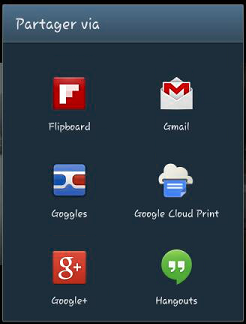
\includegraphics[scale=0.5]{images/share1}
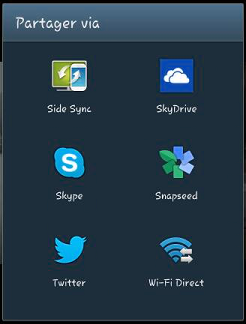
\includegraphics[scale=0.5]{images/share2}
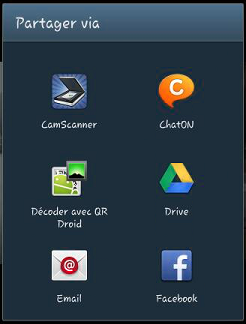
\includegraphics[scale=0.5]{images/share3}
\end{center}
\bigskip

Par exemple si l’utilisateur a installé l’application « Facebook », ce
dernier apparaîtra dans la liste ci-dessus. Si l’utilisateur n’a pas
installé « Google+ », ce dernier ne sera pas dans la liste et il ne
pourra donc pas partager sur « Google+ » via ce bouton. D’un côté, si
l’utilisateur n’a pas l’application associée, cela peut signifier qu’il
n’utilise pas le réseau social concerné et donc ce ne sera pas
problématique pour lui.

\subsubsection{Évaluation sur le Google Play Store}

Un bouton a été mis en place afin de permettre à l’utilisateur qui y
clique d’arriver directement sur notre application dans le Google Play
Store pour y mettre un commentaire ainsi qu’une (bonne) note.

Ce bouton fonctionne et ouvre l’application « Google Play Store » du
téléphone. Cependant, il affiche un message d’erreur, par manque de
finitions, nous ne l’avons pas publié sur le Google Play Store.

\subsubsection{API Google+}

Pour utiliser les services d’API de Google, il faut créer une
application dans le Google API console. Ce dernier nous fournit les
informations nécessaires comme les clés pour pouvoir utiliser l’API de
Google+. Cette fonctionnalité nous a demandé beaucoup plus de temps que
prévu. En effet, nous ne nous attendions pas à une telle complexité pour
l’ajout d’un simple bouton de partage sur Google+. Il est nécessaire
d’écrire plusieurs centaines de lignes pour faire fonctionner ce bouton
de partage et malgré de nombreux tests, nous n’avons jamais réellement
réussi à le faire fonctionner.

\subsubsection{API Facebook}

Pour utiliser l’API de « Facebook », nous avons dû utiliser le compte
d’un des membres de l’équipe afin qu’il ait un compte « Facebook
developer » et ainsi pouvoir enregistrer l’application au sein de
Facebook et obtenir l’ID de l’application. Encore une fois nous sommes
étonnés par la complexité de l’ajout d’un simple bouton de partage via un
SDK. Nous avons pratiquement abouti au résultat souhaité. Lorsque
l’application Facebook n’est pas installée, le bouton génère une page
web dans une Frame fonctionnelle. Au contraire, quand l’application
Facebook est installée, le bouton déclenche l’ouverture de l’application
Facebook qui échoue à la connexion. Ce bouton n’est pas complètement
opérationnel. De plus, nous n’avons pas trouvé comment créer un bouton
« Connexion \& partage ». Visiblement selon le SDK, nous aurions été
obligés de séparer ces deux opérations.

\subsubsection{API Twitter}

Twitter n’a pas d’API pour partager l’application via un bouton dans une
application Android. Nous avons donc utilisé une autre API non
officielle qui permet d’effectuer le partage en ouvrant une page web
 dans une Frame en laissant à l’utilisateur le soin de se connecter et
 valider le message.

\subsection{Générateur de cartes}
\bigskip


Un des caractères innovant de cette application est sans nul doute le
générateur de cartes.
En effet, aucun autre jeu de type worms que nous avons trouvé dans le
store ne permettait de générer ses propres cartes. Pour cela, nous avons
pensé une application pouvant prendre des photos, et permettant de jouer
dessus, selon le même principe que la réalité augmentée mais en version
statique.
\bigskip

Au début, nous voulions uniquement utiliser l'image en fond et rajouter
par-dessus l'image de la terre sur laquelle les joueurs se poseraient.
Puis, après discussion, nous avons trouvé qu'il serait plus amusant de
considérer l'image en tant que sol pour qu'on puisse la détruire avec
les impacts des armes.
\bigskip

On a donc implémenté la possibilité d'utiliser la caméra intégrée pour
prendre des photos. Cette étape qui devait être simple s'est avérée être
bien plus compliquée que prévu.

En effet, les informations publiées dans
la documentation de l'API Android ne sont pas respectées. Lors de
l'appui sur le bouton pour prendre une photo, un callback est appelé
lorsque l'image est disponible en format dit « raw » et transmis en
argument, puis un autre est appelé un peu plus tard lorsque l'image est
disponible en format compressé jpeg et le transmet en argument.

Dans les nouvelles versions d'Android, ces callbacks sont toujours
appelés pour des raisons de rétrocompatibilité, mais le callback
d'image « raw » renvoie null comme argument. Alors que nous voulions
utiliser un format « raw » pour choisir le format, la compression des
données, les données brutes n'étaient jamais disponibles. Aucune
documentation ne spécifiait que dans les dernières versions d'Android,
aucune image brute n'était plus disponible. Nous avons donc utilisé les
images déjà compressées.
\bigskip

L'étape suivante était d'implémenter la possibilité de dessiner sur
l'image ou sur un fond bleu de la terre, et de l’effacer pour remettre
du ciel. Le plus intuitif selon nous était d'utiliser de la
transparence, les zones transparentes représentant le ciel, et les zones
non transparentes représentant la terre.

Nous avons décidé d'utiliser
plusieurs tailles de brosses afin de faire des dessins plus ou moins
précis. Lors d’un appui sur l’écran, nous dessinons alors un cercle
dont la taille dépend de la taille de brosse choisie, et nous le
colorions en couleur terre, le tour du cercle en couleur herbe, ou alors
nous appliquons une transparence si l’outil d’effacement est
sélectionné.
\bigskip

Lors des tests, nous nous sommes aperçus que pendant le temps de
traitement durant lequel nous dessinions le cercle et appliquions les
transformations, l’application était bloquée et ne répondait plus aux
actions de l’utilisateur. Une des conséquences est que nous n’obtenions
pas de traits continus lorsque l’on effectuait un glissé sur l’écran.
Dès lors, une de nos priorités a été de traquer les moindres
ralentissements de l’application lors du dessin, ce qui fût une tâche
difficile et longue.
\bigskip


La dernière chose que nous avons implanté, c’est un algorithme
permettant à l’utilisateur de séparer automatiquement la photo en zone
de ciel et zone de terre. Cette fonctionnalité permet en effet de
sélectionner les zones claires, et d’appliquer de l’alpha dessus afin de
les transformer en ciel. Pour cette fonctionnalité, plusieurs
algorithmes ont été essayés.

\subsubsection{Seuillage fixe:}

On choisit une valeur de densité que l’on appelle seuil, puis on
parcourt l’image en calculant la densité de chaque pixel. Si cette
densité est inférieure à la valeur de seuil, le pixel sera transformé
en ciel et si elle est supérieure au seuil, le pixel sera conservé tel
quel.
\bigskip

Cet algorithme a l’avantage d’être simple et peu coûteux en temps et
ressources, mais les résultats produits étaient très aléatoires et peu
esthétiques.

En effet, on ne peut prédire si l’image sera plutôt claire
ou plutôt sombre. Si le seuil choisit est trop bas et l’image est
sombre, la carte ne contiendra pas assez de ciel et les personnages ne
pourront pas se déplacer.

Au contraire, si le seuil choisit est trop
haut et que l’image est claire, la carte finale ne contiendra pas de
terre et les personnages tomberont instantanément.

\subsubsection{Seuillage dynamique :}

On procède tout d’abord à un calcul de la densité moyenne de l’image.
Cette densité moyenne indiquera au programme si l’image est plutôt
sombre ou plutôt claire. Nous prenons alors cette densité moyenne pour
valeur de seuil et utilisons la même technique que dans l’algorithme
précédent.
\bigskip

Cette technique est très peu coûteuse mais ne donne pas de résultats
très esthétiques

\subsubsection{K-means:}

On débute en prenant deux pixels aléatoire p1 et p2, on calcule leurs
densités d1 et d2. Ces deux densités forment alors la base de deux
ensembles e1 et e2. On parcourt ensuite l’ensemble des pixels et pour
chaque pixel p, on calcule sa densité d, et on le place dans un des
ensembles selon le critère suivant :
\bigskip

\begin{itemize}
\item si la distance |d-d1| est inférieure à la distance |d-d2|, on le
placera dans l’ensemble e1,
\item si la distance |d-d1| est supérieure à la distance |d-d2|, on le
placera dans l’ensemble e2.
\end{itemize}
\bigskip

Une fois tous les pixels de l’image parcourus, on calcule la densité
moyenne de chacun des pixels appartenant aux ensembles, d1’ et d2’.

Ces deux densités servent alors de base à deux nouveaux ensembles e’1 et e’2.
On réitère un nombre fixe de fois jusqu’à obtenir deux densités moyennes
finales f1 et f2.

La plus faible de ces densités sera prise pour densité
du ciel et la plus élevée pour densité de la terre. On regroupe alors de
la même manière que précédemment les pixels selon leur densité : proche
de la densité du ciel ou de la terre. On applique enfin un alpha aux
pixels dont la densité est plus proche de la densité du ciel.
\bigskip

Cet algorithme donne de bons résultats quel que soit le type de photo,
mais est extrêmement coûteux en temps surtout si le matériel possède un
faible processeur

\subsubsection{Technique hybride :}

D’après les tests effectués sur les autres algorithmes, nous avons alors
imaginé un algorithme hybride essayant d’allier des résultats esthétiques
et peu coûteux.
\bigskip

L’algorithme imaginé sépare les pixels de l’image en deux classes, la
classe du ciel et la classe de la terre à la façon de l’algorithme
K-means (celui qui donnait les meilleurs résultats).

Nous partons de
l’hypothèse que le ciel est plus clair que la terre. On effectue un
premier parcours de l’image en cherchant le point le plus clair (le
moins dense) et le point le plus sombre (le plus dense) de l’image. Nous
séparons ensuite les pixels de l’image en deux classes : la classe
sombre et la classe claire, de la même façon que l’algorithme K-means,
en calculant la distance entre la densité de chaque pixel et les points
sombres ou clairs. Puis nous appliquons de l’alpha sur les points les plus clairs.
\bigskip

Cet algorithme était beaucoup moins coûteux que K-means et donnait des
résultats semblables. Cependant, on pouvait observer des
artefacts : certains pixels clairs qui
apparaissaient au milieu de zones sombres se voyaient appliquer un
alpha, ce qui donnait des résultats peu esthétiques. Pour l’améliorer,
nous avons décidé de diminuer la résolution de calcul. Lors de la phase
de séparation, au lieu de traiter pixel par pixel, nous traitons des
blocs de plusieurs pixels, calculant la moyenne de densité des blocs
avant de les classer dans l’une ou l’autre des catégories.
\bigskip

Donnant des résultats très esthétiques avec un temps de calcul suffisamment 
réduit, nous avons décidé d'utiliser cet algorithme.

\subsection{Proof-Of-Concept (POC)}
\bigskip


Notre intention dans ce projet était d’ajouter un maximum d'éléments
intéressants dans cette application. Vu que nous étions bloqués sur
certains problèmes techniques du moteur graphique, nous avons réalisé
des POC afin de voir la complexité de réalisation de certains éléments.

Nous avons testé l’intégration du son, du vibreur et de l’accéléromètre.
Ces éléments sont disponibles dans l’application mais pas toujours
utilisés comme on pourrait s’y attendre.

\subsubsection{le son}

Nous avons intégré le son sur un bouton du jeu : le bouton qui devait
permettre de mettre le jeu en pause émet un son lorsqu’on appuie dessus.
Par défaut le son est désactivé dans les paramètres du jeu, il faut
l’activer pour pouvoir le tester.

\subsubsection{le vibreur}

Nous avons intégré le vibreur du téléphone à chaque déclenchement
d’explosion. Par défaut le vibreur est désactivé dans les paramètres du
jeu, il faut l’activer pour pouvoir le tester.

\subsubsection{l’accéléromètre}

Nous avions comme idée, de faire des armes de différents types dans le
jeu. Une de ces armes aurait dû être un missile téléguidé par
l’accéléromètre du téléphone. Pour ce faire, nous avons réalisé une page
de test depuis le menu principal de l’application en clinquant sur
« Test du gyro ». Cette petite flèche rose orientée, tourne en fonction
des mouvements et de l’inclinaison du téléphone. Par manque de temps, nous
n’avons malheureusement pas eu l’occasion de l’intégrer au projet.

\subsection{Problèmes rencontrés et solutions appliquées}
\bigskip


\subsubsection{Problème de mémoire limitée}

Sur certains appareils, il n’est pas possible de stocker plus de deux ou
trois images volumineuses en même temps en mémoire. De ce fait il n’est
pas possible d’annuler les actions lors de la prise de photo avec
l’appareil photo.

\subsubsection{Android 2.3.x}

Le SDK utilisé était assez ancien, ce qui permet de couvrir un maximum
de téléphones. Mais cela nous a également empêché d’utiliser les
nouvelles  fonctionnalités des SDK plus récents. Il a donc fallu créer
à la main des méthodes intégrées dans le SDK 4.0 par exemple.

Ce SDK contient également peu de composants graphiques complexes ; il a
fallu contourner cette absence.

\subsubsection{Moteur graphique}

Nous avons eu beaucoup de difficultés à avoir un moteur graphique
fonctionnant de manière correcte. Les premières tentatives permettait
bien d’afficher les objets, de déplacer et de zoomer la carte, mais
elles étaient complexes et nous paraissaient difficilement utilisables ;
elles étaient peu compréhensibles et très peu maniables. Il a fallu
plusieurs versions pour obtenir une version qui au final n’était pas
totalement satisfaisante. Le développement de jeux vidéo sur Android a
été bien plus complexe que nous l’avions imaginé. De plus l’accent étant
mis au fil des semaines sur l’interface graphique, en effet son absence
était bloquante pour beaucoup d’autres parties du projet, il a fallu que
d’autres membres du projet s’y intéressent afin d’obtenir le plus
rapidement possible un environnement de test réaliste.
\newpage

\newpage

\section{Qualité et tests}
\bigskip


\subsection{Qualité code source avec Sonar}
\bigskip


\begin{figure}[h]
\begin{wrapfigure}{l}{30mm}

\includegraphics{images/sonar_logo}
\end{wrapfigure}
\noindent
Nom du logiciel : SonarQube (anciennement SonarSource)\\
Site internet : \url{http://www.sonarqube.org/}\\
Licence : OpenSource\\
Fonctionnalités : Analyse de la qualité du code source\\
Langages supportés : Sous formes de plugins\\
\bigskip
\end{figure}
\noindent
Sonar est un logiciel OpenSource qui permet de faire de l’analyse sur
la qualité du code source d’une application. C’est une application qui
regroupe des librairies de contrôle de code existant sûr et qui fournit
les violations à ces règles ainsi que des statistiques sur le projet.
Ces informations permettent d’assurer un suivi sur la qualité de
l’application et permettent ainsi de réduire le risque de bugs tout en
ayant un code source relativement propre.

\subsection{Matériels de test}
\bigskip


De nombreux tests ont été effectués de manière régulière sur une large
gamme de téléphones et tablettes :

\begin{center}
\begin{tabular}{|c|c|c|}
\hline
{\bf Nom} & {\bf Version Android} & {\bf Taille de l'écran}\\
\hline
Samsung Galaxy S4 & 4.2.2 & 1920 x 1080\\
\hline
Samsung Galaxy S3 & 4.1.2 & 1280 x 720\\
\hline
Samsung Galaxy Ace 2 & 2.3.6 & 800 x 480\\
\hline
Samsung Galaxy Y & 2.3.6 & 320 x 240\\
\hline
Nexus S & 4.1.2 & 800 x 480\\
\hline
Google Nexus 7 & 4.2.2 & 1280 x 736\\
\hline
\end{tabular}
\end{center}
Ces tests ont permis de détecter certains problèmes complètement
invisibles sur d’autres mobiles. Ces problèmes étaient principalement
dus à :
\bigskip
\begin{itemize}
\item la gestion des ressources mémoire (250Mo à 2Go de RAM selon
les mobiles)
\item la version d’Android (2.3.6 à 4.2.2)
\item la taille de l’écran qui varie énormément et qui complique
l’affichage des éléments graphiques
\end{itemize}
\bigskip

Nos tests n’ont pas été poussés comme nous l’aurions souhaité. Le
projet n’était pas entièrement abouti, nous avons que faiblement fait
tester notre application par des personnes tierces.

\subsection{Tests du singe}
\bigskip


Le SDK de Android intègre la possibilité de faire des tests du singe
monkey test) sur une application Android. Le fonctionnement consiste à
démarrer une machine virtuelle Android avec l’application à tester, puis
de lancer une commande qui va exécuter au choix un certain nombre
d'opérations aléatoires sur la machine.

Étant donné qu’une machine virtuelle est démarrée, nous pouvons voir
comment se comporte l’application selon les différentes actions du
singe. Nous avons également accès aux logs de l’application et du
téléphone.

\begin{center}

\includegraphics[scale=0.8]{images/monkey}
\end{center}

L’objectif de ces tests, est de repérer :
\begin{itemize}
\item si le singe arrive à faire des actions théoriquement interdites
\item s’il arrive à faire planter l’application (ce qui entraîne l’arrêt
de l’application)
\item s’il arrive à produire des comportements jugés « bizarre » dans
ses actions.
\end{itemize}
Ces tests peuvent également être qualifiés de « stress tests » puisque
le singe fait un très grand nombre d’actions par seconde et peut donc
détecter des problèmes qu’un utilisateur lambda ne produira pas.

Grâce à ces tests, nous avons donc repéré quelques défauts dans notre
application que nous avons répertoriés ou directement corrigés.

\subsection{Tests unitaires}
\bigskip


Nous avons tenté de mettre des tests unitaires dans notre application
au mois de janvier. Mais nous ne sommes pas allés au bout de notre
intégration, car nous avons remarqué que plusieurs facteurs rentraient
en jeu.

\subsubsection{Problème de temps}

Début janvier, nous avions déjà remarqué des difficultés d’utilisation
du moteur graphique. Or la création de tests unitaires demande un temps
de développement non négligeable.

\subsubsection{Pas de nécessité}

Dans la mesure où cette application ne demande que très peu de code ou
de fonctionnalités de pur développement (presque tout le code est en
interaction avec l’interface), il n’y a que très peu de fonctions à
couvrir avec des tests unitaires. Dans le cas d’une librairie, il aurait
été bien plus judicieux de mettre des tests en place.

De plus, nous possédons déjà une assurance qualité avec Sonar.

Toutes ces raisons nous ont confortés dans notre décision de nous passer
de tests unitaires.

\newpage

\section{Statistiques}
\bigskip


\subsection{Statistiques générales}
\bigskip


Voici quelques statistiques sur notre projet :
\begin{itemize}
\item 5171 lignes de code java (sans les lignes vides, ni les
commentaires, ni les librairies)
\item 1740 lignes d’interfaces graphiques en XML
\item 787 lignes de commentaires dans le code Java (soit 13,2\% de
commentaires)
\item 0\% de duplication de code
\item 97,3\% de taux de conformité dans Sonar
\item 321 commits
\item 67 classes réparties dans 4 packages
\end{itemize}

\subsection{Statistiques détaillés issues de Sonar}
\bigskip


Ci-dessous, nous allons détailler quelques informations issues de Sonar

\subsubsection{Index de qualité}


\begin{center}
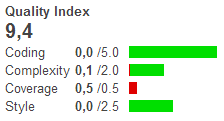
\includegraphics[scale=0.7]{images/quality_index}
\end{center}

Cette note s’explique principalement par le fait que nous n’avons pas
effectué de tests unitaires.

\subsubsection{Alertes remonté par Sonar}

Voici les alertes remontées par notre serveur Sonar. Dans cette fenêtre
d’historique, on peut voir les alertes en passant la souris sur le

\includegraphics[scale=0.8]{images/info_icon}.

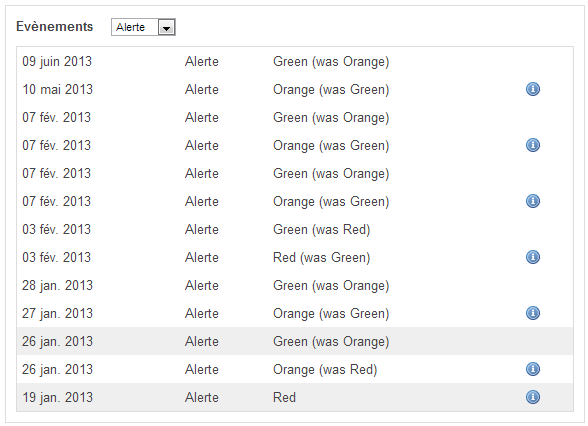
\includegraphics[scale=0.8]{images/alert1}

Dans la majorité des cas, les alertes ont permis de rétablir rapidement
la situation. La seule exception se situe entre le 10 mai et le 9 juin,
en raison du manque de documentation de l’API. Cette alerte n’était pas
spécialement importante et a pris du temps à être corrigée.

Aujourd’hui, le projet est conforme, il ne possède aucune alerte.


\includegraphics{images/alert2}

\subsubsection{Historique et évolution du projet}

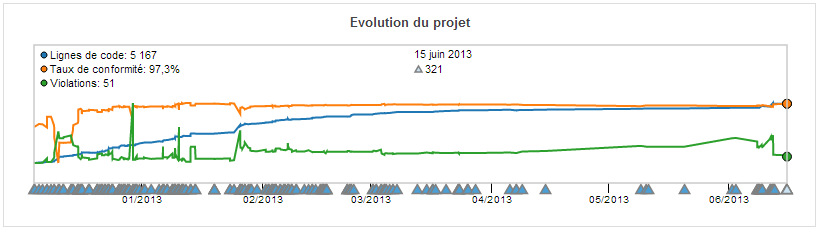
\includegraphics[scale=0.55]{images/evolution}

Sur ce graphique on voit la courbe bleue représentant le nombre de
lignes de code qui a évolué tout au long du projet. La courbe orange
représente le taux de conformité ; peu respecté au début du projet le
temps que chacun prenne conscience des standards de développement. 

La courbe verte, quant à elle, représente le nombre de violations dans
le code.

Sous le graphique, les flèches représentent les analyses de Sonar. On
remarque que le développement a été très actif au début, et plus faible
sur la fin (tout en restant actif). A noter que certains commits n’ont
pas été analysés à cause de bugs sur le serveur d’intégration.

\subsubsection{Respect des interdépendances entre packages}
%TODO : commenter un peu cette section quand même
\begin{center}
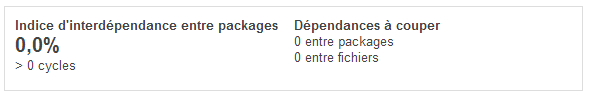
\includegraphics[scale=0.5]{images/depedencies}
\end{center}

\subsubsection{État du projet}
\begin{center}
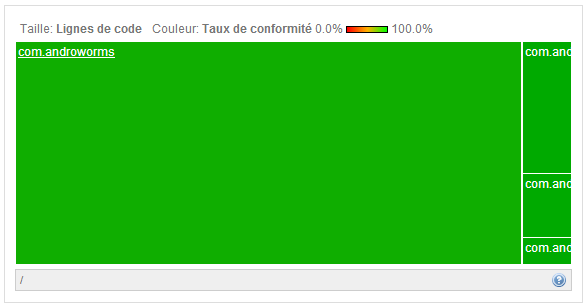
\includegraphics[scale=0.8]{images/state1}
\end{center}
Zoom sur le package com.androworms :


\begin{center}
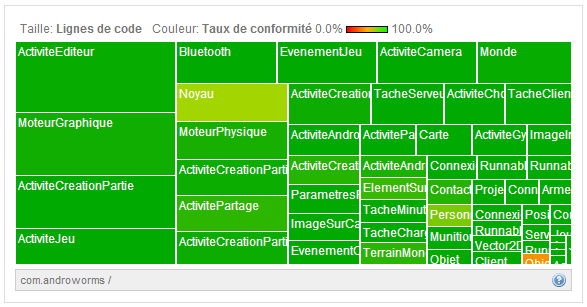
\includegraphics[scale=0.8]{images/state2}
\end{center}

\subsubsection{Qualité globale de l’application}

Le projet ne possède pas à un taux de conformité de 100\%. Analysons
ensemble pourquoi la  métrique n’est qu’à 97,3\%.


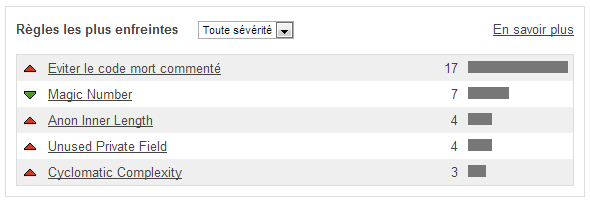
\includegraphics[scale=0.75]{images/rules}

« Éviter le code mort commenté » est assez simple à comprendre. La
règle « Magic Number », quant à elle, correspond à une présence de
nombres différents de 0, 1 et 2 directement dans les instructions. En
effet ces nombres correspondent généralement à des valeurs modifiables
leur placement dans une constante est donc souhaitable.

Les 2 règles les plus enfreintes sont des règles qui disparaissent avec
la fin du développement actif du projet. Dans la mesure où notre projet
n’a pas atteint ce point de finition, nous avons encore des violations.

\subsubsection{Statistiques SVN}

Les logs SVN sont disponibles sur notre Google Code à l’adresse suivante :

\url{https://code.google.com/p/androworms/source/list}

\bigskip

Les statistiques SVN générés par Sonar sont disponibles à l’adresse suivante :

\url{http://doc.petrolkiwi.net/dashboard/index/Androworms?did=8}


\newpage

\section{Conclusion et perspective}
\bigskip


Le développement de jeux vidéo est complexe de par les multitudes
d'interactions matérielles/logiciels qu’il comporte et y jouer n’apprend
rien sur leurs créations. De plus les appareils mobiles sont en plein
essor à travers le monde, c’est pourquoi notre projet fut orienté vers
cette architecture.

Cependant, personne de notre groupe ne possédait de compétences dans
les deux domaines explorés dans ce projet. Nous avons donc tenté de
relever ce double défi en développant un jeu similaire aux « Worms ».
Ce projet arrivant à son terme, le résultat attendu n’est
malheureusement pas celui espéré, néanmoins l’ensemble des difficultés
techniques du projet ont été réalisé. Par exemple, nous avons utilisé
les API Facebook, Google+ et Twitter comme demandé. Nous avons également
utilisé des composants spéciaux comme la caméra, le Bluetooth ou
l’accéléromètre du téléphone. En outre l’ensemble des interactions entre
les joueurs et les actions des personnages sont fonctionnelles. 

Lors de ce projet, nous avons aussi pu découvrir l’importance des
interactions entre les différentes personnes constituant notre groupe
comme la difficulté à faire un transfert de connaissance intéressant et
performant lors des réunions. Nous pensons donc, que l’apport de ce sujet
libre a été important et nous aurions aimé avoir plus de temps afin de
mener à bien ce projet.

\end{document}
